\section{Evaluations} \label{GLOBALsec:evals}

We implemented the algorithms from~\cref{GLOBALsec:methods} in the aligner \astarpa
and refer to the two of our algorithms as \SH for \sh, and \CSH for \csh. Here
we empirically compare the runtime and memory usage to the exact optimal
aligners \edlib and \wfa on both synthetic and real data. We demonstrate the
benefit of match pruning on the runtime scaling with sequence length, and the
benefits from match chaining and inexact matches on scaling to high error rates.
All code, evaluation scripts and data are available in the \astarpa repository.

\subsection{Setup} \label{sec:evals-setup}

\paragraph{Synthetic data}
Our synthetic datasets are parameterized by sequence length~$n$, induced error
rate~$e$, and total number of basepairs~$N$, resulting in $N/n$ sequence pairs.
The first sequence in each pair is uniform-random from~$\Sigma^n$. The second is
generated by sequentially applying~$\lfloor e{\cdot} n\rfloor$ edit operations
(insertions, deletions, and substitutions with equal~$1/3$ probability) to the
first sequence. Introduced errors can cancel each other, making the
\emph{divergence}~$d$ between the sequences less than~$e$. Induced error rates
of $1\%$, $5\%$, $10\%$, and~$15\%$ correspond to divergences of $0.9\%$,
$4.3\%$, $8.2\%$, and~$11.7\%$, which we refer to as $1\%$, $4\%$, $8\%$,
and~$12\%$.

\paragraph{Human data}
We use two datasets%
of ultra-long Oxford Nanopore Technologies (ONT) reads of the human genome: one
without and one with genetic variation. All reads are $500\mbox{--}1100\kbp$
long, with mean divergence around $7\%$. The average length of the longest gap
in the alignment is
$0.1\kbp$ for ONT reads, and $2\kbp$ for ONT reads with genetic
variation~(detailed statistics in~\cref{tab:hg}).
The reference genome is
CHM13~(v1.1)~\citep{nurk2022complete}. The reads used for each dataset are:

\begin{itemize}
  \item \emph{ONT}: $50$ reads sampled from those used to assemble
        CHM13.
  \item \emph{ONT with genetic variation}: $48$~reads from another
        human~\citep{bowden2019sequencing}, as used in the \wfa
        paper~\citep{marco2022optimal}.
\end{itemize}

\paragraph{Algorithms and aligners}
We compare \SH, \CSH, and \GCH as implemented in \astarpa%
to the state-of-the-art exact aligners \wfa and \edlib. We also compare to
\dijkstra and to variants without pruning, and without diagonal transition. We
exclude \seqan and \parasail since they are outperformed by \wfa and
\edlib~\citep{marco2021fast}.

\paragraph{\astarpa parameters}
We run all aligners with unit edit costs with traceback enabled, returning an
alignment. In \astarpa we fix $r{=}2$ (inexact matches) and seed length
$k{=}15$. Both are a trade-off: inexact matches and lower $k$ increase the
heuristic potential to efficiently handle more divergent sequences, while too
low $k$ gives too many matches.

\paragraph{Execution}
We use
\pabench
on Arch Linux on an \texttt{Intel Core i7-10750H} processor with $\qty{64}{GB}$
of memory and $6$ cores, without hyper-threading, frequency boost, and CPU power saving
features. We fix the CPU frequency to \texttt{2.6GHz}, limit the memory usage to
$\qty{32}{GiB}$, and run $1$ single-threaded job at a time with niceness $-20$.

\paragraph{Measurements}
\pabench first reads the dataset from disk and then measures the wall-clock time
and increase in memory usage of each aligner. Plots and tables refer to the
average alignment time per aligned pair. Best-fit polynomials are calculated via
a linear fit in the log-log domain using the least squares method.


%\input{\dir/app-tools}
\begin{table*}[t]
    \ra{0.8}
    \centering

    \renewrobustcmd{\bfseries}{\fontseries{b}\selectfont}
    \renewrobustcmd{\boldmath}{}

	\sffamily
    \setlength{\tabcolsep}{3pt}
    \begin{tabular}{
        @{}
        rl %l
        S[table-format=2.2, detect-weight, mode=text]
        S[table-format=3.2, detect-weight, mode=text]
        S[table-format=4.1, detect-weight, mode=text]
        S[table-format=4.0, detect-weight, mode=text]
        l
        S[table-format=3.1, detect-weight, mode=text]
        S[table-format=3.1, detect-weight, mode=text]
        S[table-format=3.1, detect-weight, mode=text]
        S[table-format=3.1, detect-weight, mode=text]
        @{}
    }
%    \addlinespace[-\aboverulesep]
%    \cmidrule[\heavyrulewidth]{2-10}
    & & \multicolumn{4}{ c }{\textbf{Runtime} [\unit{s}]}& & \multicolumn{4}{ c }{\textbf{Memory} [\unit{MB}]}\\
    \cmidrule{3-6} \cmidrule{8-11}
%\hspace{12.5em} 
    & \textbf{Aligner} $e=$ & {$1\%$}  & {$5\%$} & {$10\%$} & {$15\%$} & & {$1\%$} & {$5\%$} & {$10\%$} & {$15\%$} \\
    \cmidrule{1-11}
    \rowcolor{gray!10}
    \edlibsymbol                & \edlib      & 206  & 839  & 1653 & 3073 &&  \bfseries 102 &  \bfseries 106 & \bfseries 105 & \bfseries 106 \\
    \wfasymbol                  & \wfa        & 56.9 & 806  & 2799 & 5492 &&  148  &  168  & 181 & 190 \\
    \rowcolor{gray!10}
    \shsymbol~\shsymbolsq       & \textbf{\astarpa}    & \bfseries 1.41 & \bfseries 2.79 & 82.5 & \text{ML} && 434   & 548   & 4759 & \text{ML} \\
    \cshsymbol~\cshsymbolsq     & \textbf{\astarpa} (chain)   & 1.60 & 2.98 & \bfseries 12.3 & \bfseries 220 && 436   & 543   & 2369 & 4696 \\
    \cmidrule{1-11}
    \end{tabular}
	\caption[Performance comparison of global alignment tools]{Runtime and
      memory comparison on \textbf{synthetic sequences} of length $n{=}10^7\bp$
      for various error rates. ML stands for exceeding the memory limit
      of~$\qty{30}{GB}$. Note that we run our \A heuristics with exact
      matches~(\shsymbol~\cshsymbol) when $e{\leq}5\%$, and with inexact
      matches~(\shsymbolsq~\cshsymbolsq) when $e{\geq}10\%$.}
	\label{GLOBALtab:evals}
\end{table*}

\subsection{Comparison on synthetic data} \label{GLOBALsec:evals-comparison-synthetic}

Here we compare the runtime scaling and performance of the exact optimal
aligners on synthetic data.
\cref{GLOBALsec:techniques} compares the effects of pruning and inexact matches,
whereas~\cref{GLOBALsec:expanded} compares \SH and \CSH in terms of the number of
expanded states.

\paragraph{Scaling with sequence length}
% figs: better scaling => faster for long
First, we compare the aligners by runtime scaling with sequence length $n$ for
various error rates $e$ (\cref{GLOBALfig:scaling-n}). As expected from the theoretical
analysis, \edlib and \wfa scale approximately quadratically regardless of the
error rate. Unlike them, \SH and \CSH scale subquadratically which explains why
they are faster for long enough sequences.

% for low error rates
More specifically, for low error rates ($e{=}1\%$ and $e{=}5\%$), both \SH and
\CSH with exact matches scale near-linearly with sequence length (best
fit~$n^{1.08}$ for \mbox{$n{\le}10^7$}), and the benefit from chaining is
negligible.

% for high error rates
For high error rates ($e{\geq}10\%$) and large $n$, the need to match the seeds
inexactly causes a significant number of off-path matches. These off-path
matches lower the value of the heuristics and prevent the punishment of
suboptimal paths. This causes \SH to expand a super-linear number of states
(\cref{GLOBALsec:expanded}). Chaining the matches enforces them
to follow the order of the seeds, which greatly reduces the negative effects of
the off-path matches, leading to only linearly many expanded states.
Nevertheless, the runtime scaling of \CSH
is super-linear as a result of the increasing fraction of time (up to $93\%$ for
$n{=}10^7$) spent on reordering states because of outdated $f$ values after
pruning.

%(TODO: high variance; more seqs needed)
\paragraph{Performance}
\cref{GLOBALtab:evals} compares the runtime and memory of \astarpa with match
pruning to \edlib (based on banding, exponential search, bit-parallel) and \wfa
(based on diagonal transition and divide \& conquer) for aligning a single pair
of sequences of length $n{=}10^7$. \A with \CSH (\cshsymbol~\cshsymbolsq) is
more than $250$ times faster than \edlib and \wfa at $e{=}5\%$. For low error
rate ($e{\leq}5\%$), there is no significant performance difference between \SH
(\shsymbol~\shsymbolsq) and \CSH. The memory usage of \astarpa for $e{\leq}5\%$
is less than $\qty{600}{MB}$ for any $n$. At $e{=}15\%$, \CSH uses at most
$\qty{4.7}{GB}$ while \SH goes out of memory ($\geq\qty{30}{GB}$) because there
are too many expanded states to store.

   
%& \A, match-pruning, \sh                      
%& \A, match-pruning, \csh                     

\subsection{Comparison on real data} \label{GLOBALsec:evals-comparison-hg}

\begin{figure}[H]
  \centering
  \subfloat[CHM13: ONT read errors]%
  {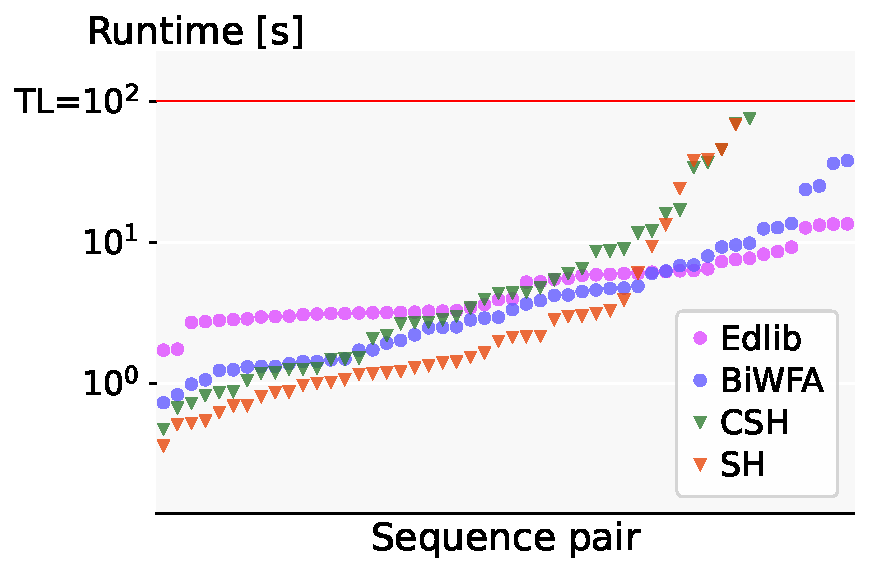
\includegraphics[width=0.48\linewidth]{imgs/fig7/human_sorted_chm13.pdf}}
  \hfill
  \subfloat[NA12878: ONT read errors + biological variation]%
  {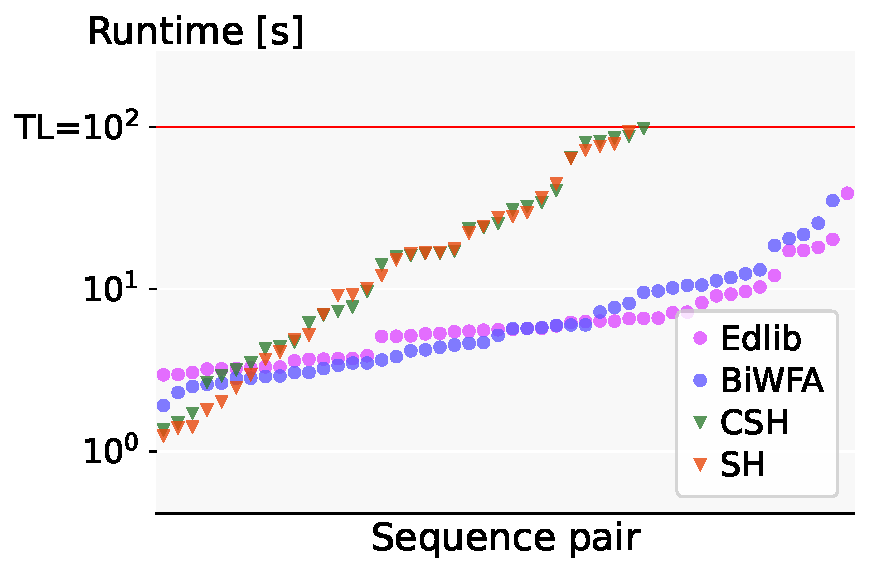
\includegraphics[width=0.48\linewidth]{imgs/fig7/human_sorted_na12878.pdf}}
  \caption[Runtime per sequence (real data)]{Log plot comparison of the
  aligners' runtime on \textbf{real data}. The data points for each individual
  aligner are sorted by alignment time. Alignments that timed out after $100$
  seconds are not shown.}
  \label{GLOBALfig:human-results}
\end{figure}

In this section we compare the exact optimal aligners on long ONT reads from our
human datasets~(\cref{GLOBALfig:human-results}). With the presented minimalistic
features, \astarpa aligns some sequences faster than \wfa and \edlib, but the
high runtime variance makes it slower overall~(\cref{GLOBALsec:variation-human-results}).

% heuristics vs biwfa/edlib
On the dataset without biological variation \datasetOne, \SH is faster than \wfa
and \edlib on $58\%$ of the alignments ($29$ of $50$). On the dataset with
biological variation \datasetTwo, \SH outperforms \wfa and \edlib on $17\%$ of the
alignments ($8$ of $48$) and in other cases is over an order of magnitude
slower. In both datasets, \SH and \CSH time out for the sequences with the
highest edit distances, because they have an error rate larger than the
heuristic can handle efficiently~($e\geq r/k=2/15=13.3\%$).

% SH vs CSH
\CSH usually explores fewer states than \SH since \csh dominates
the \sh. However, in certain cases \CSH is slower than \SH since needs more time
to update the heuristic after pruning (Step 3$'$ in \cref{GLOBALsec:compute-csh}).
%, and %spends up to $98\%$ of its time on this.


\subsection{Effect of pruning, chaining, and inexact matches}\label{GLOBALsec:techniques}

\begin{figure}[t]
  \centering
  \subfloat[The effect of pruning on the runtime scaling with $n$ ($e{=}5\%$,
      $k{=}15$, exact~matches). Note that \SH and \CSH coincide almost exactly.]
      {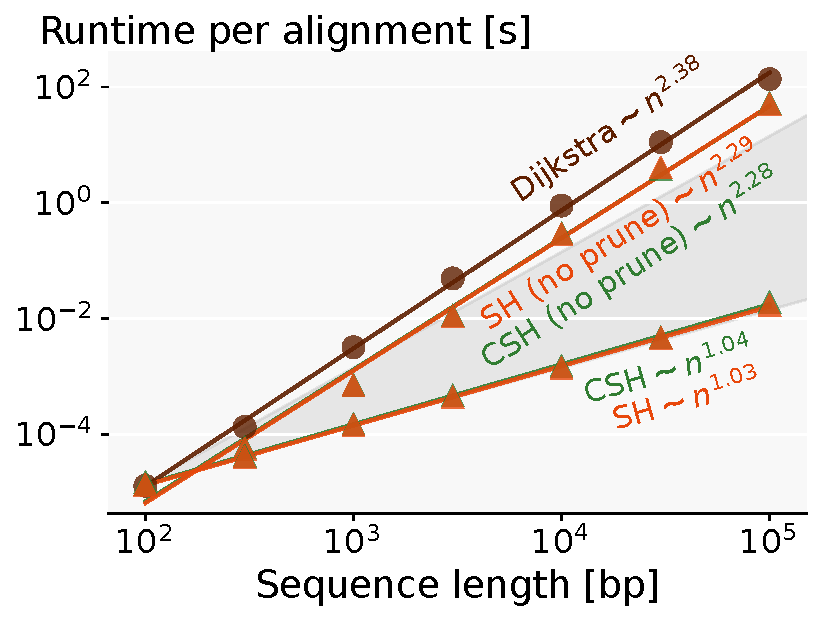
\includegraphics[width=0.45\linewidth]{imgs/fig5/scaling_n_labels.pdf}\label{GLOBALfig:scaling_n}}
  %\hfill
  \subfloat[The effect of chaining and inexact matching on the runtime scaling
  with $e$ ($n{=}10^4$, $k{=}9$, averaged over $100$ alignments).]
  {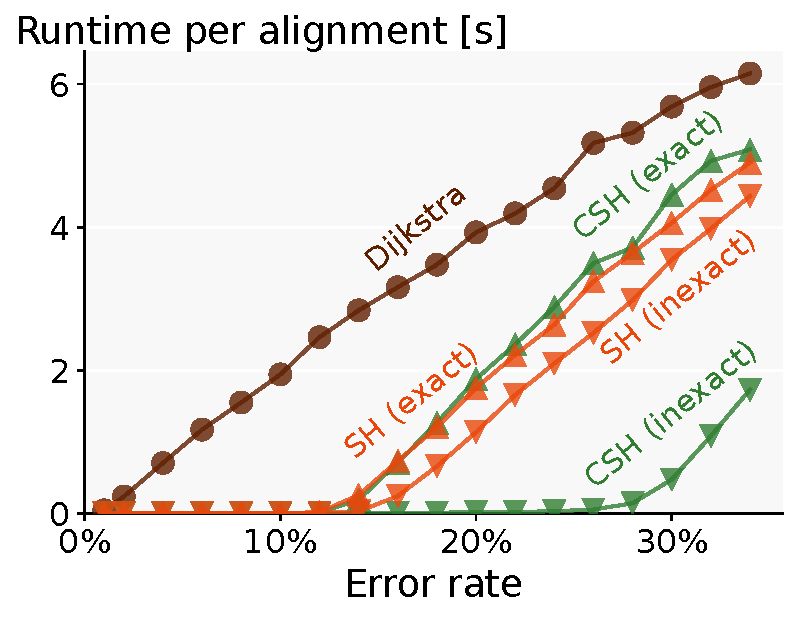
\includegraphics[width=0.45\linewidth]{imgs/fig5/scaling_e_labels.pdf}\label{GLOBALfig:scaling_e}}

  \caption[The effects of pruning, inexact matching, and chaining on runtime
   scaling with length and error rate]{The effects of seed heuristic
   optimizations on runtime scaling (\textbf{synthetic data}).}
  \label{GLOBALfig:scaling}
\end{figure}


The optimizations and generalizations of the seed heuristic~(\cref{GLOBALsec:methods})
impact the performance in a complex way. Here we aim to provide intuitive
explanations~(\cref{GLOBALfig:scaling}).

\paragraph{Pruning enables near-linear scaling with length}
\cref{GLOBALfig:scaling_n} shows that match pruning has a crucial effect on the
runtime scaling with length for both \SH and \CSH. Essentially, this
optimization changes the quadratic runtime to near-linear runtime. The pruned
variants of \SH and \CSH are averaged over $\lfloor 10^7 / n \rfloor$ sequence pairs,
while the no-prune variants and \dijkstra are averaged over $\lfloor 10^5 / n
\rfloor$ pairs.

\paragraph{Inexact matching and match chaining enable scaling to high error rates}
\cref{GLOBALfig:scaling_e} shows that inexact matches can tolerate higher error rates.
Because of the larger number of matches, chaining is needed to preserve the
near-linear runtime. There are two distinctive modes of operation: the runtime
is close to constant up to a certain error rate, after which the runtime grows
linearly in $e$. Thus, our heuristics can direct the search up to a certain
fraction of errors, after which does a \dijkstra-like exploration step for each
additional error. A reasonable quantification of the effect of different
optimizations is to mark the error rate at which the heuristic transfers to the
second (slow) mode of operation. For $n{=}10^4$ and $k{=}9$, \dijkstra starts a
linear exploration at $e{=}0\%$, \SH and \CSH with exact matches start at around
$12\%$, \SH with inexact matches start at around $14\%$, and \CSH with inexact
matches start at around $27\%$.

%The jumps in the graphs, especially visible for \dijkstra, are caused by layers
%of memory caches being exhausted.

% We choose $n{=}10^4$ since it is not near the limit for any of \sh and \csh. In
% order to highlight the difference between \sh and \csh, we choose a smaller
% value $k{=}2$, which is suboptimal for longer $n$.

%Supplementaries
%- Expanded states/band, Expanded states 1.00 scaling, h0 for SH+pruning and CSH+pruning for different e
%In the supplementaries~\cref{GLOBALsec:supplementaries} we study in detail the
%scaling of \sh and \csh with $n$ and $\spot$.
%- h0 approximate $72\%$ of $e$
%\paragraph{Internal for \sh}

\subsection{Expanded states and equivalent band} \label{app:expanded}

\begin{figure*}[t]
  \centering
  \subfloat[$d{=}1\%$, exact matches]{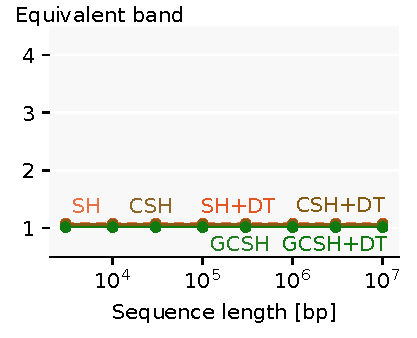
\includegraphics[scale=0.55]{plots/band_e0.01.labels.pdf}
  \label{fig:band-1}}
  \hfill
  \subfloat[$d{=}4\%$, exact matches]{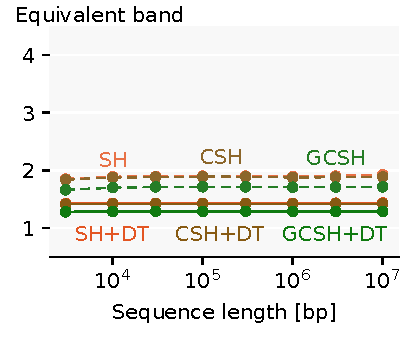
\includegraphics[scale=0.55]{plots/band_e0.05.labels.pdf}
  \label{fig:band-5}}
  \hfill
  \subfloat[$d{=}8\%$, inexact matches]{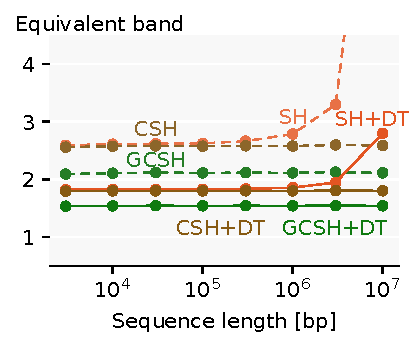
\includegraphics[scale=0.55]{plots/band_e0.10.labels.pdf}
  \label{fig:band-10}}
  \hfill
  \subfloat[$d{=}12\%$, inexact matches]{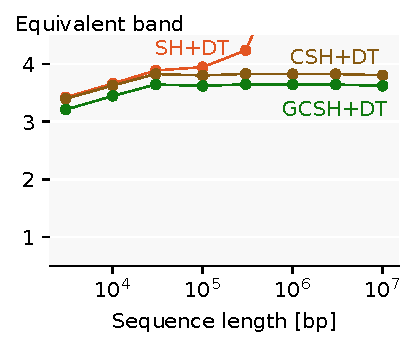
\includegraphics[scale=0.55]{plots/band_e0.15.labels.pdf}
  \label{fig:band-15}}%
  \caption[Band scaling with sequence length on synthetic data]{\textbf{Equivalent band scaling with sequence length on synthetic data.}
    ($k{=}15$, $r{=}2$ for $d{\geq}8\%$). The equivalent band is the number of
    expanded states per bp for aligning synthetic sequences. Averages are over
    total $N{=}10^7\bp$. At $d{=}12\%$, the bands of non-DT methods are $\geq
    3\times$ wider.}
  \label{fig:band}
\end{figure*}

The main benefit of an \A heuristic is a lower number of expanded states, which
translates to faster runtime. Instead of evaluating the runtime scaling with
length (\cref{fig:tools}), we can judge how well a heuristic
approximates the edit distance by directly measuring the \emph{equivalent band}
(\cref{fig:band}) of each alignment: the number of expanded states divided by
sequence length $n$, or equivalently, the number of expanded states per base pair.
The theoretical lower bound is an equivalent band of $1$, resulting from
expanding only the states on the main diagonal.

The equivalent band tends to be constant in $n$, indicating that the number of
expanded states is linear on the given domain. The equivalent band of \SH starts
to grow around $n\geq 10^6$ at divergence $d{=}8\%$, and around $n\geq 10^5$ at
$d{=}12\%$. Because of the chaining, \CSH and \GCH cope with spurious matches
and remain constant in equivalent band (i.e. linear expanded states with $n$).
The equivalent band for \GCH is slightly lower than \CSH due to better
accounting for indels. The DT variants expand fewer states by skipping
non-farthest reaching states.

\subsection{Human data results}\label{app:human}

\begin{table}[H]
  \centering
  \sffamily
  \small
  \tabcolsep=0.11cm
  \begin{tabular}{
    @{}
    l
    S[table-format=2]
    S[table-format=3]
    S[table-format=3]
    S[table-format=3]
    S[table-format=1.1]
    S[table-format=1.1]
    S[table-format=2.1]
    S[table-format=1.2]
    S[table-format=1.1]
    S[table-format=2]
    @{}
    }
    \toprule
    &
    & \multicolumn{3}{c}{\textbf{Length} [\kbp]}
    & \multicolumn{3}{c}{\textbf{Divergence} [$\%$]}
    & \multicolumn{3}{c}{\textbf{Max gap} [\kbp]}
    \\
    \cmidrule(lr){3-5} \cmidrule(lr){6-8} \cmidrule(lr){9-11}
    \textbf{Dataset}
    & {\!\!\textbf{Cnt}} &
    {\small min} & {\small \!mean} & {\small max} &
    {\small min} & {\small \!mean\!} & {\small max} &
    {\small min} & {\small \!mean\!} & {\small max} \\
    \midrule
    ONT & 50
     & 500 & 594 & 849 & 2.7 & 6.3 & 18.0 & 0.02 & 0.1 & 1 \\
    ONT+gen.var.\!\! & 48
     & 502 & 632 & 1053 & 4.4 & 7.4 & 19.8 & 0.05 & $\mathbf{1.9}$ & $\mathbf{42}$ \\
    \bottomrule
  \end{tabular}
  \caption[Human datasets statistics.]{\textbf{Human datasets statistics.} ONT reads only include short
    gaps, while genetic variation also includes long gaps. \textbf{Cnt}: number of
    sequence pairs. \textbf{\mbox{Max gap}}: longest gap in the reconstructed
    alignment.}
  \label{tab:hg}
\end{table}

\begin{figure*}[t]
  \centering
  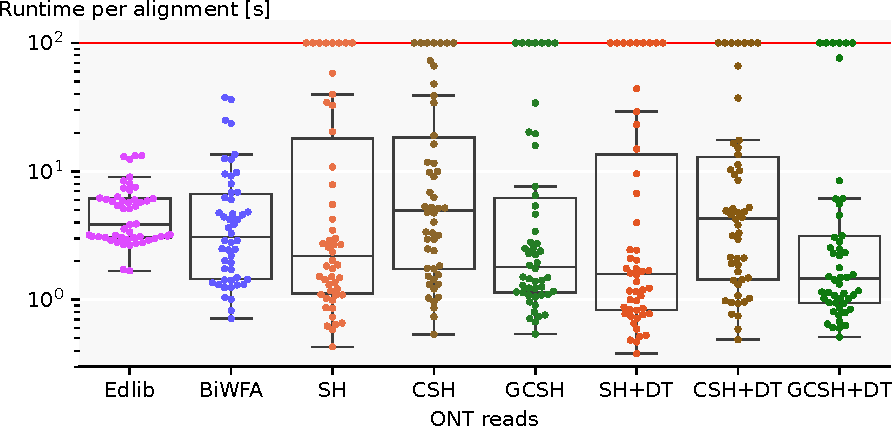
\includegraphics[scale=0.55]{plots/real_full_without_bio_var.pdf}\\
  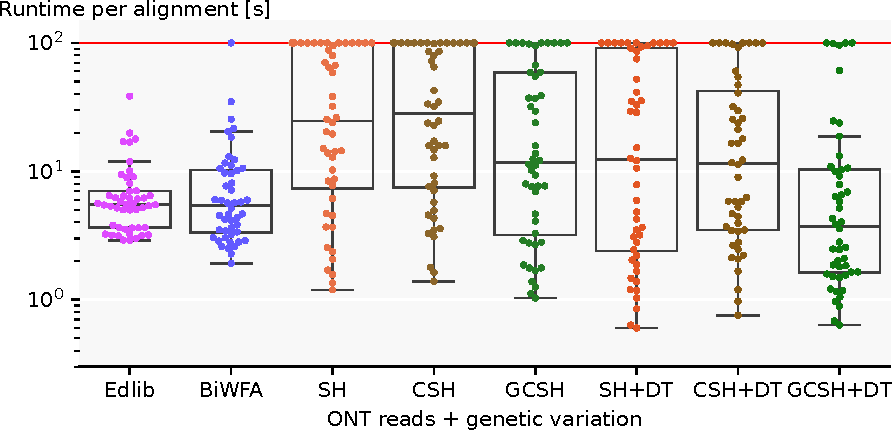
\includegraphics[scale=0.55]{plots/real_full_with_bio_var.pdf}%
  \caption[Runtime on long reads of human data]{\textbf{Runtime on long reads of
    human data} (logarithmic, $\geq 500\kbp$). Each dot corresponds to an
    alignment of a sequence pair. The ONT reads are without (top) and with
    (bottom) genetic variation. Runtime is capped at $\qty{100}{s}$.}
  \label{fig:human-full}
\end{figure*}

Statistics on our human data are presented in~\cref{tab:hg}. We compare all our
heuristics in~\cref{fig:human-full}.

For ONT reads without genetic variation, \SH is faster than other methods in
median, but slower for sequences with high divergence and larger gaps.
\CSH is slightly slower than \SH due to additional bookkeeping without
significant benefit for the heuristic. Penalizing indels with \GCH improves
performance several times.

When genetic variation is included, \SH and \CSH do not sufficiently penalize
long gaps, and \A with \GCH estimates the remaining edit distance significantly
better. The diagonal transition optimization considerably speeds up the
alignment of long indels where the search regresses to quadratic.

\subsection{Complex alignments}\label{GLOBALsec:limitations}

\begin{figure}[t]
  \centering
  \subfloat[High error rate]
    {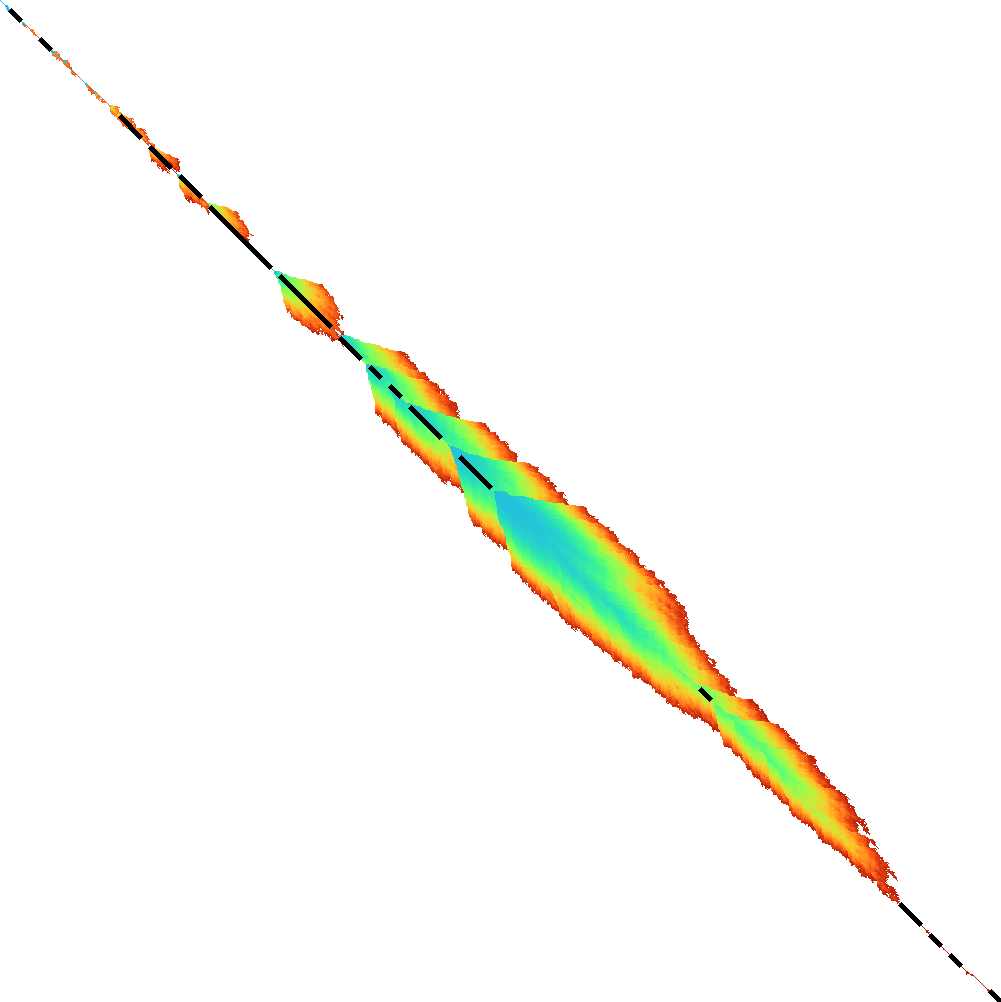
\includegraphics[height=0.31\linewidth]{imgs/fig8/high-error-rate.png}\label{GLOBALfig:high_error_rate}}
  %\hfill
  \subfloat[Long indel]
    {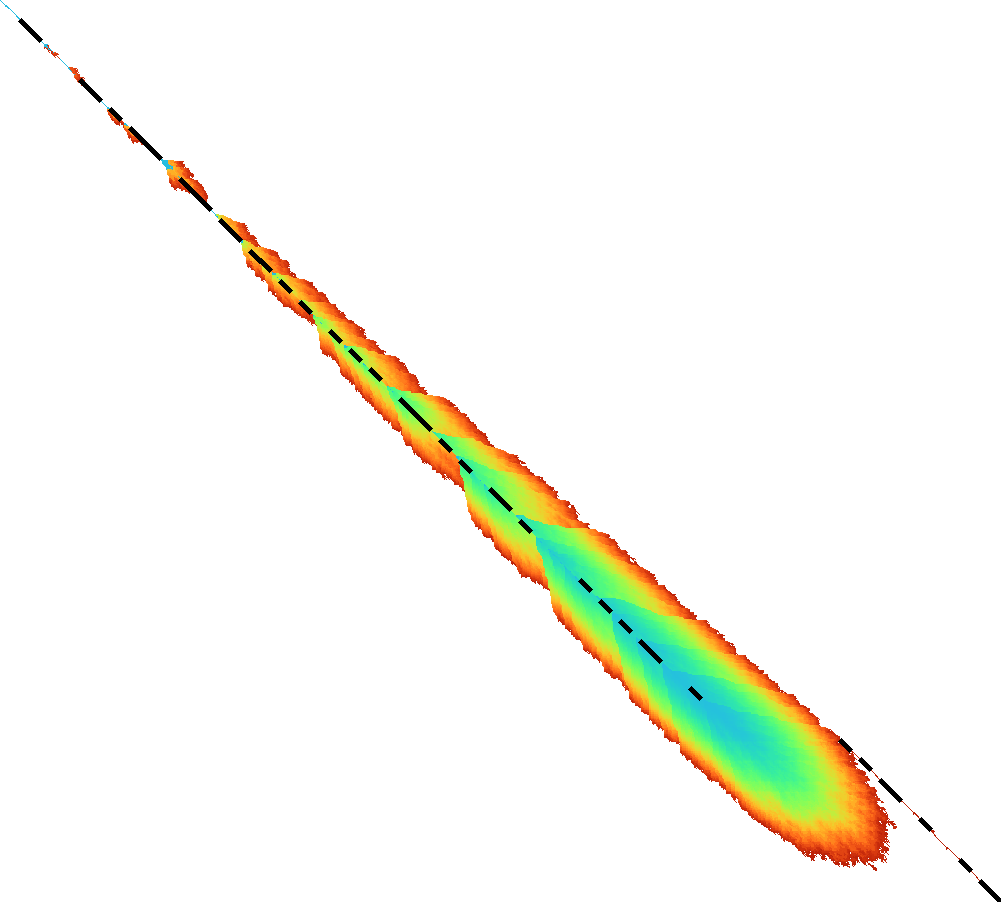
\includegraphics[height=0.31\linewidth]{imgs/fig8/deletion.png}\label{GLOBALfig:deletion}}
  %\hfill
  \subfloat[Short repeats]
    {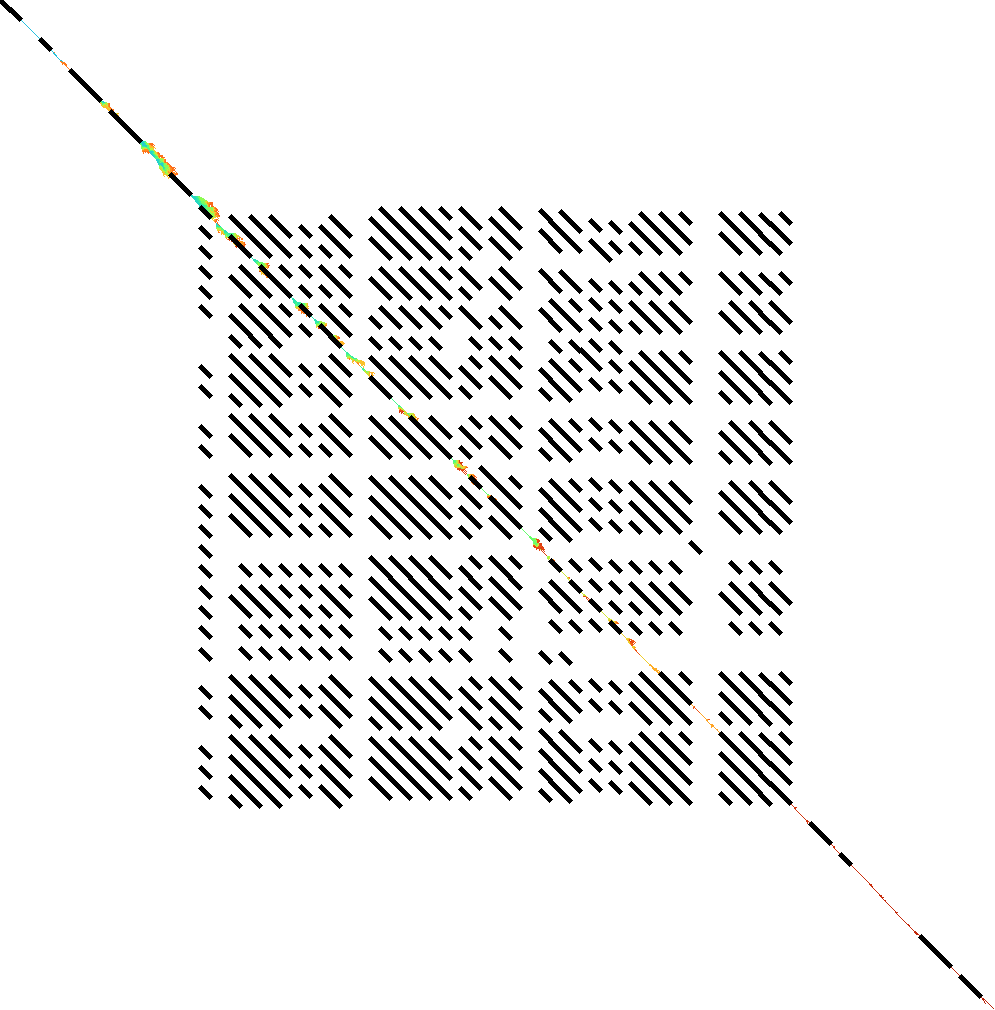
\includegraphics[height=0.31\linewidth]{imgs/fig8/repeats.png}\label{GLOBALfig:repeats}}
  \caption[Expanded states for various complex cases]{Expanded states by \CSH
  ($r{=}2$, $k{=}10$) in complex cases. The aligned pairs of \textbf{synthetic
  sequences} ($n{=}1000$) have $8\%$ uniformly random errors and contain (a) a
  region of length $200$ with larger error rate ($e{=}50\%$) than the heuristic
  can efficiently account for, (b) a deletion of length $100$, and (c) $60$
  mutated copies of a pattern of length $10$. Seed matches are shown in black
  and occur on the best paths and in the repeated region. The order of expansion
  is shown by the color gradient from blue to red.}
  \label{GLOBALfig:limitations}
\end{figure}

Our algorithm finds optimal alignments very efficiently when both the sequence
and the errors are uniformly random and the error rate is
limited~(\cref{GLOBALsec:evals}). Nevertheless, since the alignment problem is
fundamentally unsolvable in strictly subquadratic time~\citep{backurs2015edit},
there are sequences which cannot be aligned fast. We give three cases
(\cref{GLOBALfig:limitations}) for which the performance of our approach
degrades (possibly up to quadratic).

\begin{enumerate}
  \item \emph{High error rate.}
        When the error rate becomes too high (larger
        than $r/k$), seeds can not increase the heuristic enough
        penalize all errors. Each unpenalized error increases $f$ and needs more
        states to be searched, similar to \dijkstra.
        This can be mitigated by using shorter seeds and/or inexact matches, at
        the cost of introducing more matches.
  \item \emph{Long indel.}
        If there is a long insertion or deletion, the
        search has to accumulate the high cost for the long indel.
        Our heuristics do not account for long indels, and hence the search
        needs to expand states until the end of the gap is reached. Again, this
        causes a big increase of $f$ and a search similar to \dijkstra.
        This may be improved in future work by introducing a \emph{gap-cost} term to the \csh
        that penalizes gaps between consecutive matches in a chain.
  \item \emph{Short repeats.}
        When a short pattern repeats many times, this can result in a quadratic
        number of matches. This makes the corresponding seeds ineffective for
        the \sh, and slows down the computation and pruning of the \csh.
        This can be partially mitigated by increasing the seed length and/or
        exact matches, at the cost of reducing the potential of the heuristic.
        Alternatively, seeds with too many matches could be completely ignored.
\end{enumerate}

